\documentclass[greek]{beamer}
%\usepackage{fontspec}
\usepackage{amsmath,amsthm}
\usepackage{unicode-math}
\usepackage{xltxtra}
\usepackage{graphicx}
\usetheme{CambridgeUS}
\usecolortheme{seagull}
\usepackage{hyperref}
\usepackage{ulem}
\usepackage{xgreek}
\usepackage{pgfpages}
%\setbeameroption{show notes on second screen}
%\setbeameroption{show only notes}

\setsansfont{Noto Serif}

% \newtheorem{definition}{Ορισμός}

\title{Συναρτήσεις}
\subtitle{Αντίστροφη}
\author[Λόλας]{Κωνσταντίνος. Λόλας}
\date{}

\begin{document}

\begin{frame}
 \titlepage
\end{frame}

\section{Θέμα Α}
\begin{frame}
 \begin{itemize}
  \item $Α_1$ γ $\qquad Α_2$ δ $\qquad Α_3$ γ $\qquad Α_4$ β
  \item $Λ \qquad Σ \qquad Λ \qquad Σ \qquad Σ$
 \end{itemize}
\end{frame}

\section{Θέμα Β}
\begin{frame}{Β1 - (i)}
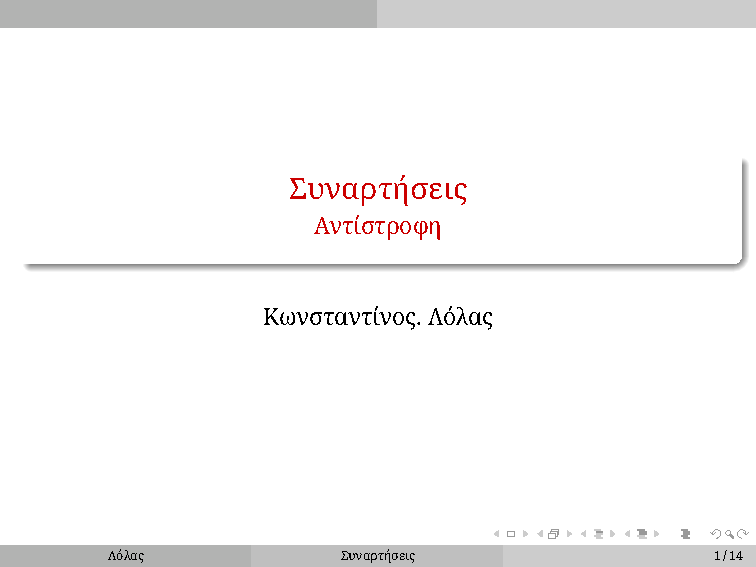
\includegraphics[width=0.35\textwidth]{"images/1.3.4 Μονοτονία.png"}<1>

 \begin{onlyenv}<2>
  \begin{gather*}
   Σ\overrightarrow{F}=\overrightarrow{0}\implies \overrightarrow{W}=-\overrightarrow{F}_{ελ} \\
   W=F_{ελ}\implies mg=k\cdot Δl_0  \\
   Δl_0=\frac{mg}{k}=Α_1 \quad (1)
  \end{gather*}
  Ασκώντας τη δύναμη $\overrightarrow{F}$, η Θ.Ι. της ΑΑΤ συμπίπτει με τη θέση φυσικού μεγέθους του ελατηρίου. Εφόσον ξεκινά από την ηρεμία, η θέση έναρξης αυτής, είναι ακραία. Άρα $$Α_2=Δl_0=\frac{mg}{k} \quad (2)$$
  $$(1),(2)\implies Α_1=Α_2$$
 \end{onlyenv}
\end{frame}

\begin{frame}{Β2 - (ii)}
 \begingroup
 \tiny% \small in 11pt base font is 10pt
 Η παροχή από κάθε οπή είναι σταθερή: $$Π=\frac{V}{Δt}\implies V=Π\cdot Δt$$
 Όταν είναι ανοιχτή μόνο η οπή (1): $$V=Π_1\cdot Δt=Αv_1\cdot Δt_1 \quad (1)$$
 Ταχύτητα εκροής: $$v_1=\sqrt{2g\left(H-\frac{5H}{6}\right)}=\sqrt{2g\frac{H}{6}}=\sqrt{g\frac{H}{3}}$$
 Όταν είναι ανοιχτές και οι δύο οπές (1), (2):
 \begin{gather*}
  V=V_1+V_2=Π_1\cdot Δt_2+Π_2\cdot Δt_2=Α\cdot v_1\cdot Δt_2+Α\cdot v_2\cdot Δt_2 \quad (2) \\
  v_1=\sqrt{g\frac{H}{3}} \qquad v_2=\sqrt{2g\left(H-\frac{H}{3}\right)}=\sqrt{2g\frac{2H}{3}}=2\sqrt{g\frac{H}{3}} \Rightarrow v_2=2v_1 \\
  Αv_1\cdot Δt_1 = Α\cdot v_1\cdot Δt_2+Α\cdot v_2\cdot Δt_2 \Rightarrow Δt_1=Δt_2+2Δt_2=3Δt_2\Rightarrow \frac{Δt_2}{Δt_1}=\frac{1}{3}
 \end{gather*}
 \endgroup
\end{frame}

\begin{frame}{Β3 - (iii)}
 \begingroup
 \tiny% \small in 11pt base font is 10pt
 $$K_1=\frac{P_1^2}{2m_1}$$
 $$K_1'=\frac{\left(\frac{P_1}{5}\right)^2}{2m_1}\frac{1}{25}\frac{P_1^2}{2m_1}=\frac{1}{25}K_1$$
 $$K_{ολ(πριν)}=K_{ολ(μετά)}\Rightarrow K_1=K_1'+K_2'\Rightarrow K_2'=\frac{24}{25}K_1 \Rightarrow \frac{K_2'}{K_1}\cdot 100\%=\frac{\frac{24}{25}K_1}{K_1}\cdot 100\%=96\%$$
 \endgroup
\end{frame}

\section{Θέμα Γ}
\begin{frame}{Γ1}
 \begin{gather*}
  I=\frac{E}{R_{ΚΛ}+r}\Rightarrow I=3A
 \end{gather*}

 \begin{gather*}
  Σ\overrightarrow{F}=\overrightarrow{0}\Rightarrow \overrightarrow{F}_L=-\overrightarrow{W}\Rightarrow F_L=W\Rightarrow \\
  B\cdot I\cdot l = mg\Rightarrow B=\frac{mg}{I\cdot l}\Rightarrow B=1T
 \end{gather*}
\end{frame}

\begin{frame}{Γ2}
 \begingroup
 \tiny% \small in 11pt base font is 10pt
 Αντίσταση θερμικής συσκευής
 $$P_Σ=\frac{V_Σ^2}{R_Σ}\Rightarrow R_Σ=6Ω$$
 Στιγμιαίες τιμές
 \begin{gather*}
  Ε_{επ}=B\cdot v \cdot l \quad I_{επ}=\frac{Ε_{επ}}{R_{ολ}}=\frac{B\cdot v \cdot l}{R_{ΚΛ}+R_{1,Σ}} \quad R_{1,Σ}=\frac{R_1\cdot R_Σ}{R_1+R_Σ}=2Ω \\
  F_L=B\cdot I_{επ} \cdot l=\frac{B^2vl^2}{R_{ΚΛ}+R_{1,Σ}}
 \end{gather*}
 Αρχικά $W>F_L$, οπότε:
 $$  Σ\overrightarrow{F}=\overrightarrow{W}+\overrightarrow{F}_L\uparrow\uparrow\overrightarrow{W} \text{ δηλαδή } Σ\overrightarrow{F} \upuparrows \overrightarrow{v}$$
 Άρα επιταχυνόμενη κίνηση με στιγμιαία επιτάχυνση μέτρου:
 $$ΣF=mg-F_L=ma\Rightarrow a=g-\frac{mg-F_L}{m}=g-\frac{B^2vl^2}{m\left(R_{ΚΛ}+R_{1,Σ}\right)}$$
 Καθώς αυξάνει το μέτρο της ταχύτητας $v$, μειώνεται το μέτρο της επιτάχυνσης. Ο αγωγός αποκτά οριακή ταχύτητα όταν
 \begin{gather*}
  a=0\Rightarrow g=\frac{B^2v_{ορ}l^2}{m\left(R_{ΚΛ}+R_{1,Σ}\right)}\Rightarrow v_{ορ}=\frac{mg\left(R_{ΚΛ}+R_{1,Σ}\right)}{B^2l^2}\Rightarrow v_{ορ}=12m/s
 \end{gather*}
 \endgroup

\end{frame}

\begin{frame}{Γ3}
 Τη στιγμή όπου $v=\frac{v_{ορ}}{2}=6m/s$
 \begin{gather*}
  I'=\frac{Bvl}{R_{ολ}}=\frac{Bvl}{R_{ΚΛ}+R_{1,Σ}}=\frac{6}{4}=1,5A \\
  \frac{dP}{dt}=ΣF=mg-F_L=mg-BIl=3-1,5=1,5kg\frac{m}{s^2}
 \end{gather*}

\end{frame}

\begin{frame}{Γ4}
 Όταν $v_{ορ}=12m/s\Rightarrow I_{ορ}=\frac{Bv_{ορ}l}{R_{ΚΛ}+R_{1,Σ}}=3A$
 \begin{gather*}
  V_{ΚΛ}=V_{πολ}=I_{ορ}R_{1,Σ}=3\cdot 2=6V
 \end{gather*}
 Άρα $V_{ΜΝ}=V_{ΚΛ}=6V=V_Σ\Rightarrow$ κανονική λειτουργία
\end{frame}

\section{Θέμα Δ}
\begin{frame}{Δ1}
 \begin{gather*}
  Σ_{τ(Γ)}=0\Rightarrow W\frac{l}{2}συνφ+N_B\frac{l}{2}συνφ=T_1\frac{l}{2}ημφ \Rightarrow \\
  N_Bσυνφ=T_1ημφ-Wσυνφ \Rightarrow \\
  0,6N_B=10,5\cdot 0,8-10\cdot 0,6 \Rightarrow 0,6N_B=8,4-6\Rightarrow N_B=4N
 \end{gather*}
\end{frame}

\begin{frame}{Δ2}
 \begin{gather*}
  I_{ολ}=I_{ρ}+I_{σφ}=\frac{1}{12}M_ρl^2+m\left(\frac{l}{2}\right)^2=\frac{1}{12}\cdot 3\cdot 4 + 1\cdot 1=2kg\cdot m^2 \\
  Σ_{τ(Γ)}=I_{ολ}α_{γων}\Rightarrow mg\frac{l}{2}συνφ=I_{ολ}\cdot α_{γων}\Rightarrow \\
  10\cdot 0,6=2α_{γων}\Rightarrow α_{γων}=3rad/s^2 \\
  \frac{dL_ρ}{dt}=I_ρ\cdot α_{γων}=3kg\cdot m^2/s^2
 \end{gather*}
\end{frame}

\begin{frame}{Δ3}
 Γωνιακή ταχύτητα $ω$ ωριακά πριν φτάσει στο οριζόντιο δάπεδο
 \begin{gather*}
  E_{ολ(αρχ)}=E_{ολ(τελ)}\Rightarrow \\
  mglημφ+M_ρg\frac{l}{2}ημφ=0+M_ρg\frac{l}{2}ημφ+\frac{1}{2}I_{ολ}ω^2\Rightarrow \\
  10\cdot 2\cdot 0,8=\frac{1}{2}2ω^2\Rightarrow ω=4rad/s \\
  |\overrightarrow{L}_{πριν}|=I_{ολ}|\overrightarrow{ω}|=2\cdot 4=8kg\cdot m^2/s \\
  |\overrightarrow{L}_{μετά}|=I_{ολ}|\overrightarrow{ω}'|=2\cdot 2=4kg\cdot m^2/s \\
  Δ\overrightarrow{L}=\overrightarrow{L}_{μετά}-\overrightarrow{L}_{πριν}\Rightarrow ΔL=4-(-8)=12kg\cdot m^2/s
 \end{gather*}
\end{frame}


\begin{frame}{Δ4}
 Κύλιση χωρίς ολίσθηση
 $$v_E=0\Rightarrow v_{cm}=ωR\Rightarrow a_{cm}=a_{γων}$$
 Μεταφορική
 $$ΣF=F+T_{στ}=M_T\cdot a_{cm}$$
 Περιστροφική
 \begin{gather*}
  Σ_{τ(Ο)}=I_{τρ}\cdot a_{γων} \Rightarrow F\cdot r-T_{στ}R=\frac{1}{2}M_TR^2\cdot a_{γων}\Rightarrow \\
  F\frac{r}{R}-T_{στ}=\frac{1}{2}M_T\cdot a_{cm}
 \end{gather*}
 \begin{gather*}
  F\left(1+\frac{V}{R}\right)=\frac{3}{2}M_T\cdot a_{γων}\Rightarrow \\
  F\left(1+\frac{3}{4}\right)=\frac{3}{2}M_T\cdot a_{γων}\Rightarrow a_{γων}=\frac{7F}{6M_T}=2m/s^2
 \end{gather*}
\end{frame}

\begin{frame}{Δ5}
 $Δx_{cm}=\frac{1}{2}a_{cm}t_1^2=\frac{1}{2}\cdot 2 \cdot 4=4m$
 Μετατόπιση άκρου νήματος:
 \begin{gather*}
  Δx_z=Δx_{cm}+r\cdot Δφ=Δx_{cm}+r\frac{Δx_{cm}}{R}=Δx_{cm}\left(1+\frac{r}{R}\right)=\frac{7}{4}Δx_{cm}=7m
 \end{gather*}
 \begin{gather*}
  W_F=F\cdot Δx_z\cdot συν0^\circ=12\cdot 7=84J
 \end{gather*}
\end{frame}

\end{document}
